%% Template for MLP Coursework 3 / 18 Feb 2018 

%% Based on  LaTeX template for ICML 2017 - example_paper.tex at 
%%  https://2017.icml.cc/Conferences/2017/StyleAuthorInstructions

\documentclass{article}

\usepackage[T1]{fontenc}
\usepackage{amssymb,amsmath}
\usepackage{txfonts}
\usepackage{microtype}

% For figures
\usepackage{graphicx}
\usepackage{subfigure} 

% For citations
\usepackage{natbib}

% For algorithms
\usepackage{algorithm}
\usepackage{algorithmic}

% the hyperref package is used to produce hyperlinks in the
% resulting PDF.  If this breaks your system, please commend out the
% following usepackage line and replace \usepackage{mlp2017} with
% \usepackage[nohyperref]{mlp2017} below.
\usepackage{hyperref}
\usepackage{url}
\urlstyle{same}

% Packages hyperref and algorithmic misbehave sometimes.  We can fix
% this with the following command.
\newcommand{\theHalgorithm}{\arabic{algorithm}}


% Set up MLP coursework style (based on ICML style)
\usepackage{mlp2017}
\mlptitlerunning{MLP Coursework 3 (\studentNumber)}
\bibliographystyle{icml2017}


\DeclareMathOperator{\softmax}{softmax}
\DeclareMathOperator{\sigmoid}{sigmoid}
\DeclareMathOperator{\sgn}{sgn}
\DeclareMathOperator{\relu}{relu}
\DeclareMathOperator{\lrelu}{lrelu}
\DeclareMathOperator{\elu}{elu}
\DeclareMathOperator{\selu}{selu}
\DeclareMathOperator{\maxout}{maxout}

%% You probably do not need to change anything above this comment

%% REPLACE this with your student number
\def\studentNumber{s1738623, s1773940, s1771076}
\def\mathbi#1{\textbf{\em #1}}

\begin{document} 

\twocolumn[
\mlptitle{MLP Coursework 3: Deep Networks Music Classification Based on FMA}

\centerline{\studentNumber}

\vskip 7mm
]

\begin{abstract} 
One of Music information retrieval (MIR) problems is music automatic categorization. As a subset of machine learning (ML), deep learning (DL) often performs well in classification problems in a proper way. In this report, we build a deep learning classification model to classify the music. Also, we testify our model on EMINST dataset and explore the relationship of the data provided by the dataset named Free Music Archive (FMA). The results from the experiment show three main conclusion. First, our model is correct and performs well by on EMINST. Second, (). Third, the reason of unsatisfied performance on FMA dataset is the given data from dataset FMA is not able to represent the whole audio data. Finally, give some future plans to improve the project including extracting new features, build new models and correlating the project with recommendation systems.
\end{abstract} 

\section{Introduction}
\label{sec:intro}
Classification is the approach, which identities different subjects to specific categories, having a wide application. There are many applications based on classification like filtering the spam emails, cancer identification etc. Solving classification problems is worthy in many aspects.

As a approach of solving classification problems, machine learning (ML) can lead to a good classification result after training relative data sets in a proper way. Most of the machine learning classification methods are belong to supervised learning which uses labeled data as training data. As one of the most important machine learning method, neural network (NN) outperforms than many approaches in the early time. However, neural network using gradient descent in backpropagation may suffers from the gradients vanish after increasing the number of layers. This problems were solved by \cite{hinton2006reducing} and deep learning, a kind of multi-layer NN, became popular since then.

Deep learning(DL) is a subset of machine learning and there are three main types of learning. In a deep learning model, there are multiple layers each of whose input is from the former layer's output. Many of current deep learning models are based on Artificial neural network (ANN) which includes deep neural networks (DNNs). \cite{hinton2006reducing} A deep neural network contains many hidden layers between the input layers and output layers. One of advantages of DNNs is the ability of finding non-linear relationships which are often complex. Besides DNN, there are some other deep learning algorithms, such as Recurrent neural networks (RNNs) \cite{medsker2001recurrent} and Convolutional deep neural networks (CNNs).\cite{lawrence1997face} RNNs allows data going in any direction and are mainly used as language model. CNNs are widely used in computer vision domain.

Music information retrieval(MIR), as a branch of information retrieval(IR), is the science of retrieving information from music. There are many developed IR application in the world, for example, the text information retrieval from search engine. Unlike text information retrieval, MIR research is still not much due to many reasons. One of the reason above is MIR often requires a comprehensive background in music, psychology, machine learning etc. Another reason is the lack of numbers of large, complete and available datasets. \cite{fma}. MIR is being used widely, such as recommender systems, track separation and instrument recognition, automatic music transcription, automatic categorization, music generation etc. In this project, we mainly focus on doing classification (automatic categorization).

In the rest of the report, there are mainly eight sections. Motivation, research questions and objectives will be stated in section 2 to 4 respectively. Section 5 is  a brief introduction on FMA datasets. In methodology part (section 6), a concise conclusion of machine learning practical will be given and some novel knowledge used in our experiment will be introduced as well.  After experiments part, there is  a interim conclusion containing results analysis. At the last, future plan of the project is pointed out.

\section{Motivation}
Machine learning performs good at classification, and deep learning often has a better performance on finding non-linear relationships. Music is a kind of thing containing a lot of information which is hard to find the relative relationships inside. Therefore, compared other methods, machine learning, especially deep learning, is a suitable approach to deal with music issues. 

Besides deep learning or machine learning, music, which is a natural habit of human, has a remarkable potential market to be explored. For example, a good music classification can bring clear learning schedules for new learner. Also, music recommend systems based on personal preference will be popular because of the increasing cognition of self-value. 

Therefore, in this report, our main motivation is to find an approach based on deep learning to classify the music. However, unlike text classification based on words or image classification based on image values, music classification based on data transformed from audio contains more uncertain relationship. For example, it is clear that image values represents the color, shapes and other information of each image, so it will be certainly able to classify other images by this kind of value. However, after transforming the audio to data by one method, it is not certain to say that the transformed data contains enough information of the music to do the classification. Therefore, besides building a deep learning architecture for classification, we also need to verify the relationship between transformed data (provided by dataset) and the music categories. All the experiments are based on FMA datasets and classification accuracy is the evaluation of models.\citep{fma}


\section{Research questions} 
Unlike the wealth of other information retrieval, lacking large, complete and available datasets for MIR makes MIR research develop slow. Except for FMA dataset, other existing datasets for MIR are either in small scale or not complete. 
For example, despite containing 2524739 clips, the dataset named AcousticBrainz has no information on artists or audios. Dataset called Unique provides a more complete information, but its capacity(3115 clips) is far away from the FMA(106547 clips). \cite{fma}

\begin{table}[h!]
\centering
\begin{tabular}{*{5}{c}} \hline
dataset & clips & artists & year & audio \\ \hline
RWC & 465 & $-$ & 2001 & yes \\
CAL500 & 500 & 500 & 2007 & yes \\
Ballroom&  698& $-$ & 2004 & yes \\
GTZAN&  1000& 300 & 2002 & yes \\
MusiClef&  1355&  218 & 2012 & yes \\
Artist20&  1413& 20 &  2007&  yes \\
ISMIR2004&  1458 &  $-$ & 2004 & yes  \\
Homburg& 1886 & 1463 & 2005 & yes \\
103-Artists & 2445 & 103 & 2005 & yes \\  
Unique& 3115 & 3115 & 2010 & yes \\
1517-Artists& 3180 & 1517 & 2008 & yes \\
LMD& 3227 & $-$ & 2007 & no \\
EBallroom& 4180 & $-$ & 2016 & no\\ 
USPOP&8752  & 400 & 2003 & no \\
CAL10k& 10271 & 4597 & 2010 & no \\
MagnaTagATune& 25863 & 230 & 2009 & yes \\
Codaich& 26420 & 1941 & 2006 & no \\
FMA& 106574 & 16341 & 2017 & yes \\
OMRAS2 & 152410 & 6938 & 2009 & no \\
MSD& 1000000 & 44745 & 2011 & no \\
AudioSet& 2084320 & $-$ & 2017 & no \\
AcousticBrainz& 2524739 & $-$ & 2017 & no \\ 
\end{tabular}
\caption{Information on different datasets \citep{fma}}
\label{table:1}
\end{table}

Usually, a complete and large dataset containing more information may reveal better relationships between data by fitting them into deep networks. Therefore, compared to most of the music classification based on old datasets, our project aims at building classification model based on this new dataset. Unlike some music classification based on non-musical information like artist's name, we use the given feature extracted from audio as training data. Besides these, as mentioned before, we also want to explore the relationship between given data and categories in order to verify if the given data contains enough information to represent the audio.


\section{Objectives}
In this interim report, we mainly illustrate the relationship among the machine learning, deep learning and music information retrieval. After a comprehensive research, we have found some problems leading to several worthy research points. As the priority, we want to build a classification based on DNNs by using the FMA dataset. Besides that, there are two optional goals as well. One is finding more suitable classification models based on the FMA dataset, such as RNNs etc. The other one is trying to build a recommending model based on our classification results.


\section{Data}
The dataset in our experiment is called Free Music Archive (FMA). It is a dataset opening for free and suitable for evaluating various MIR tasks. FMA dataset contains both texture and audio content inside. For texture content encode as csv format, there are some documents recording different information about songs, albums, artists etc. For audio content encoded as mp3, there are four different size of packages, which contains 8000 tracks in 30s (7.2GiB), 25000 tracks in 30s (22GiB), 106574 tracks in 30s (93GiB) and 106574 tracks untrimmed (879GiB) respectively. 

In this report, as a mid-term report, our work is mainly about the classification issues. We extract the main text features, such as article, created date, length etc., from the dataset and split it into train set, validation set and test set. Then build different models to fit the data respectively. The evaluation of our task is accuracy of classification.

\subsection{Data Pre-processing}
The data from FMA needs to be pre-processed. As mentioned before, it has four files in metadata part. They contain the data of tracks, genres, features and echonest respectively. Since our goal in the baseline part is to verify the relationship between genres and features (we want to give the genres based on the melody of the songs), we do not need the echonest file at this stage.

To construct our training data, we first fetched the genres of each song. In the track file, some of the songs may have exact one genre, others may have more than one genres or no defined genre. Therefore, we add a new genre for those songs with more than one genre. (e.g. if there are 168 different genres in total, one song may have more than one genres (e.g. genre 16 and 32) at the same time. Therefore, we define a new genre named 169, and shift all songs belonging to both genre 16 and 32 to genre 169. This means our neural network will only be considered as correct if it predict all genres right. Then, since the genres are given by numbers defined online rather than ordered numbers (which means that the genre number is not consecutive), we went through the whole data set to reorder the genres of the songs. After that, with the proper ordered numbers, we implement the normalization on the input data set, which is the feature file. Finally, we compressed the whole data set to .npz format so that it can be used by our data providers.

\section{Methodology}
\subsection{DNN}
DNN has attracted a vast of attention due to its powerful ability on solving different kinds of machine learning problems, including music classification. With an input layer, several hidden layers and an output layer, DNN takes data into the input layer and propagate it to hidden layers, where we use sigmoid function as the activation function.
\begin{equation}
	h_ j (x) =  \frac{\mathrm{1} }{\mathrm{1} + e^{- \mathbi{W}^\top \mathbi{x} + \mathbi{b} }}
\end{equation}
Described in Eq.(2), the sigmoid function provides a reasonable gradient when processing gradient descent to train the model in a classification problem. In the output layer, we use softmax function as activation function instead, since it is the commonly used for multi-type classification. 

Although Convolution neural network (CNN) is a more effective network for a complex problem, it does not perform well with the dataset we introduced above because the $\mathsf{features.csv}$ contains different kinds of characters of the audio data such bandwidth, energy, frequency distribution, etc., which are measured in different measurements. Unlike image processing, taking the density of pixels as input, when we use different kinds of features as input to a CNN, it resulted in unreasonable prediction on the test set after training. It may be feasible to process a CNN with the original audio data, consisting of huge amounts of features in the same units so one of the further plans is to improve the performance of song classification using CNN based on original audio features. As for the baseline, handling the millions of original audio data is a complicated task and an efficient way needs to be designed carefully so we shelve it temporarily. 

\subsection{Softmax}
Softmax function is commonly used in the classification problems with more than two possible classes. In this model, because there are more than two genres of music in our dataset, we use softmax function as activation function in the output layer, giving the expression as below:
\begin{equation}
	\mathrm{softmax}(\mathbi{z})_i=\frac{e^{z_i}}{\sum_j e^{z_j}},
\end{equation}

where $i$ is the index of the genre we supposed to predict, and the denominator normalizes the probability distribution. The softmax function exponentiates the value of the linear transformation of the input, which is obtained from the last hidden layer, and then normalizes it to get ${p(y=y_i|\mathbi{x})}$. Assuming we have 10 genres to be classified, then we will get a 10-dimensional vector y consisting of the probabilities of $p(y=y_j|\mathbi{x})$, where $j$ is the index of any possible genres. The output genre with the highest probability will be compared with the target genre through cross-entropy function during the training time.

\subsection{Dropout}
In the neural network, we prefer to adopt huge amounts of parameters as input, so the model is easy to obtain accurate prediction. However, too many parameters will lead to overfitting which produces worse prediction on the test set while the training set gains a nearly perfect result. Dropout was introduced to solve the overfitting problem by randomly and temporarily remove the neurons in the layers, which also constructed several new neural networks and took the combination of the “thinned” networks to improve the performance \cite{ srivastava2014dropout}. This technique was adopted on different kinds of applications such as object classification, natural language processing, speech processing, etc., and was reported to provide a better performance on a wide domain \cite{srivastava2014dropout}. However, adding dropout to a model takes a long time since each “thinned” network tends to update the parameter independently, making the parameter updating noisily. Therefore, the model needs additional techniques to speed up.

\subsection{Adam optimization}
As stochastic gradient descent (SGD) has become a most famous optimization method in traditional machine learning \cite{kingma2014adam}, several deep learning experiments for different applications also achieve great success with SGD \cite{deng2013recent, krizhevsky2012imagenet, hinton2006reducing, hinton2012improving, graves2013speech}. However, SGD might slow down and get involved into a complicated route when the objective function contains data subsampling and some kinds of noise sources such as dropout regularization, as mentioned above. \cite{hinton2006reducing, kingma2014adam}. Therefore, more efficient optimizations need to be implemented to speed up the gradient descend processing in the specific cases. In this model, we adopt Adam, which combines the advantages of AdaGrad \cite {duchi2011adaptive} and RMSProp \cite{tieleman2012lecture}, to improve the computation efficiency. In addition to the good performance on sparse data and non-stationary settings, Adam updates the weights in the network within a bounded variation so the algorithm could find the optima. The algorithms of Adam could be formally described using the following equations:
\begin{eqnarray}
	M_i(t)=\alpha M_i(t-1)+(1-\alpha)g_i(t) \\
    S_i(t)=\beta S_i(t-1)+(1-\beta)g_i(t)^2 \\
    \Delta w_i(t)=\frac{-\eta}{\sqrt{S_i(t)}+\epsilon}M_i(t)
\end{eqnarray}
Mostly, the parameter variation was constrained below the stepsize $\alpha$, which could be understood as ignoring the observed gradient $g$, if $g$ is much farther than that the current weight values. Furthermore, Adam provides an efficient optimization using less memory than normal SGD methods.

\section{Experiments}
After the data pre-processing, we started to implement our baseline experiments. Our main idea is to test the data set with some normal deep neural networks (DNN) we have built during coursework 1 and 2. The reason why we choose only DNN to perform our baseline experiments is  that DNN has been well tested and understood by all of us. Meanwhile, we are not familiar with the data set. If there are some unexpected errors in the results, we can focus on solving the data set problems rather than worrying about both neural network problems and data set problems.

In this section, we will present our baseline experiments in time line order. We will first introduce the parameters we used to set up the DNNs. Then, we will describe our three group of baseline experiments and what we learned from them.

\subsection{Neural network structure}
Our DNN structure is quite simple. We used leaky-ReLU as the activation function in the neural network. We chose the Adam optimizer as our optimizer. We also defined the loss as the "softmax cross entropy with logits". We also include the batch normalization and dropout layer in our DNN. The dropout rate is set to 0.2. The learning rate, hidden layer number and the number of neurons in the hidden layer will be varied during the experiments.

After we constructed our neural network, we tested it on the EMINST data set with learning rate is 0.2, hidden layer is 3 with each layer has 500 neurons. The results are shown as following:

\begin{figure}[h]%
\centering
\subfigure[Error]{%
\label{fig:lr0.02}%
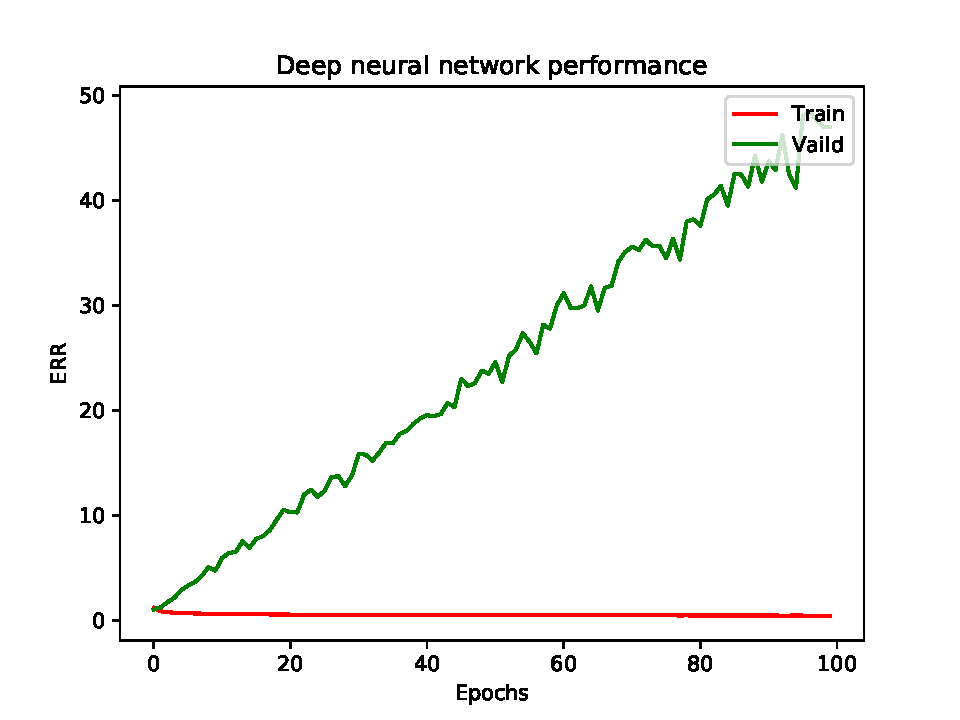
\includegraphics[height=1.25in]{Figs/St_ERR_plots_L2_N200.pdf}}%
\subfigure[Accuracy]{%
\label{fig:lr0.04}%
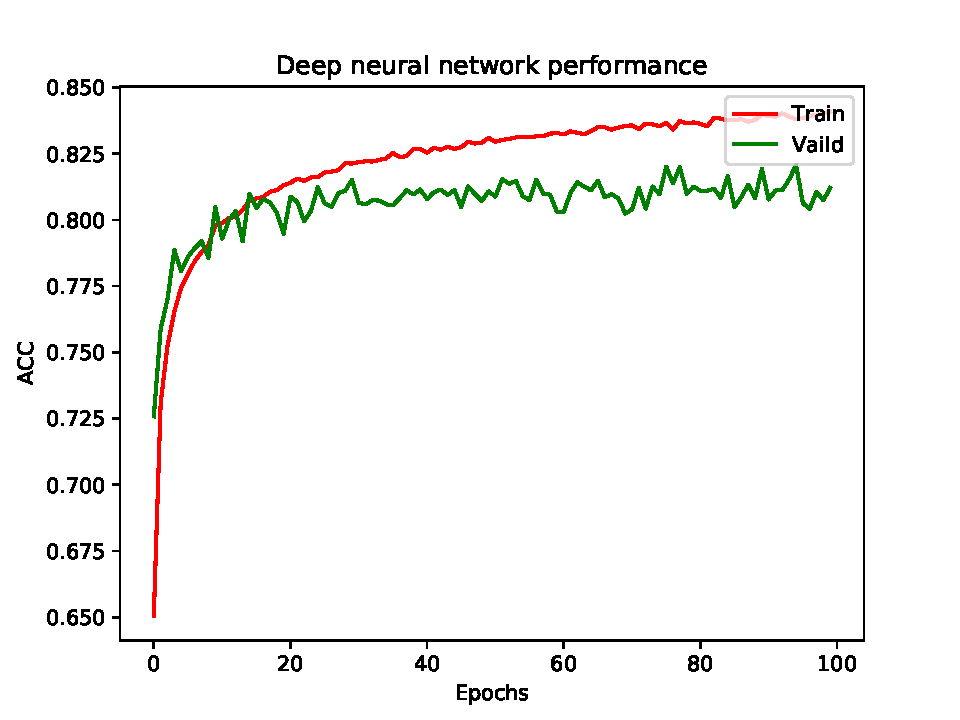
\includegraphics[height=1.25in]{Figs/St_ACC_plots_L2_N200.pdf}}%
\qquad
\caption{The EMINST on DNN}
\label{fig:NNstucture}
\end{figure}

Which shows that our neural network is constructed correctly.

\subsection{Experiments with full data}
After the neural network testing, we then provide the FMA data set to our DNN. We varied the hidden layer numbers to be 2, 3, 4 with the number of neurons in each hidden layer to be 200, 400, 600 and 800 respectively. Each neural network will be trained in 100 epochs. Which means we have $3 \times 4 \times 100 = 1200$ epochs in total. The results are shown as following:

\begin{figure}[h]%
\centering
\subfigure[Error of Train]{%
\label{fig:lr0.02}%
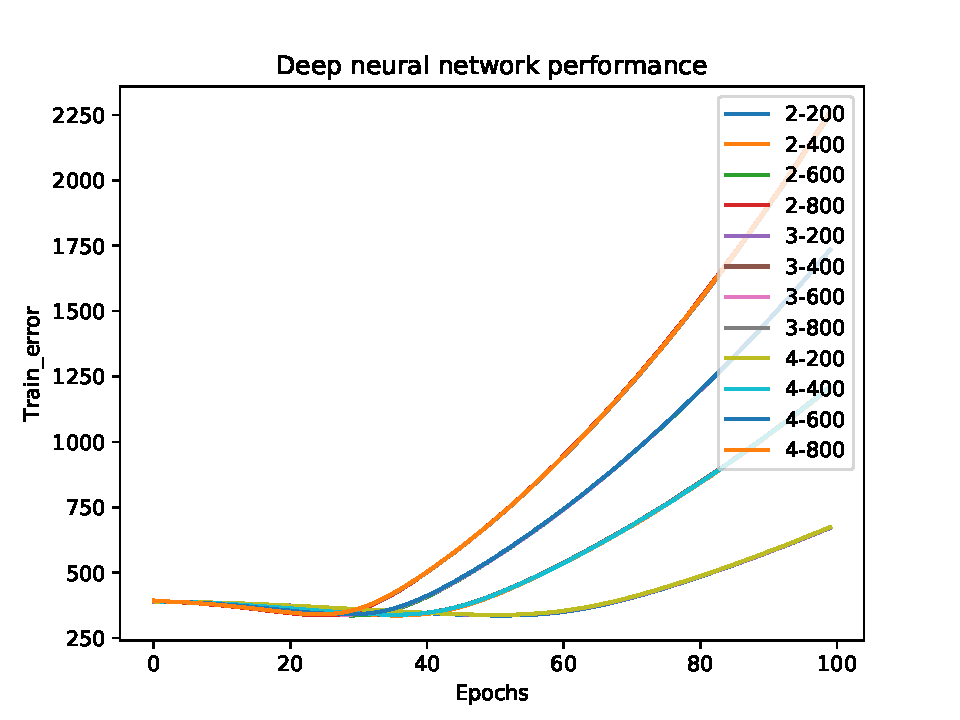
\includegraphics[height=1.25in]{Figs/AL_Train_error_plots_L2_N3.pdf}}%
\subfigure[Accuracy of Train]{%
\label{fig:lr0.04}%
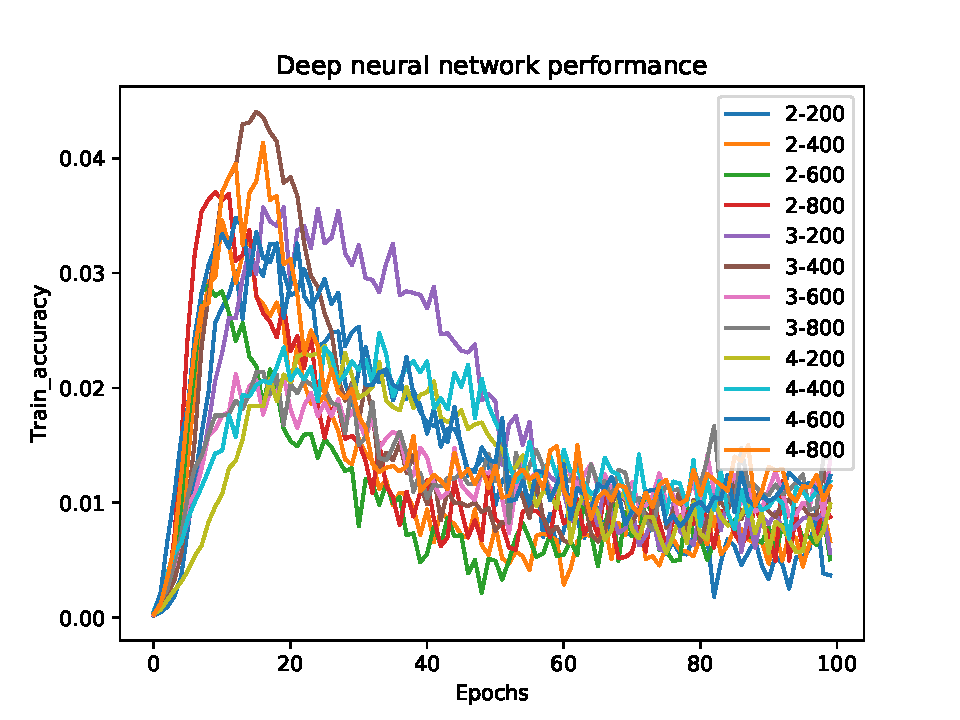
\includegraphics[height=1.25in]{Figs/AL_Train_accuracy_plots_L2_N3.pdf}}%
\qquad
\subfigure[Error of Valid]{%
\label{fig:lr0.06}%
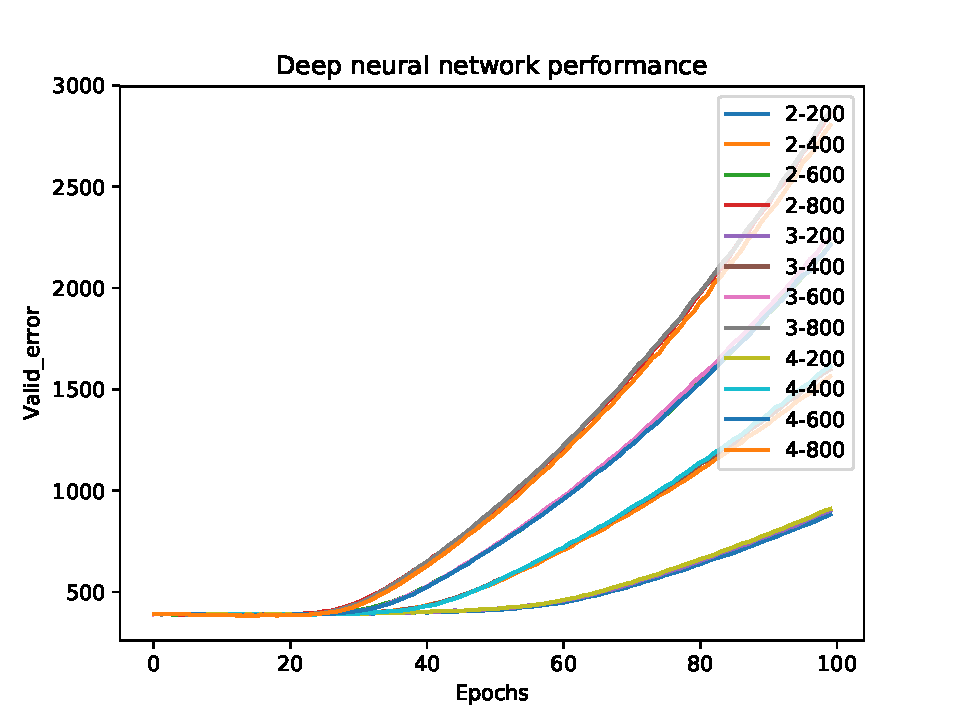
\includegraphics[height=1.25in]{Figs/AL_Valid_error_plots_L2_N3.pdf}}%
\subfigure[Accuracy of Valid]{%
\label{fig:lr0.08}%
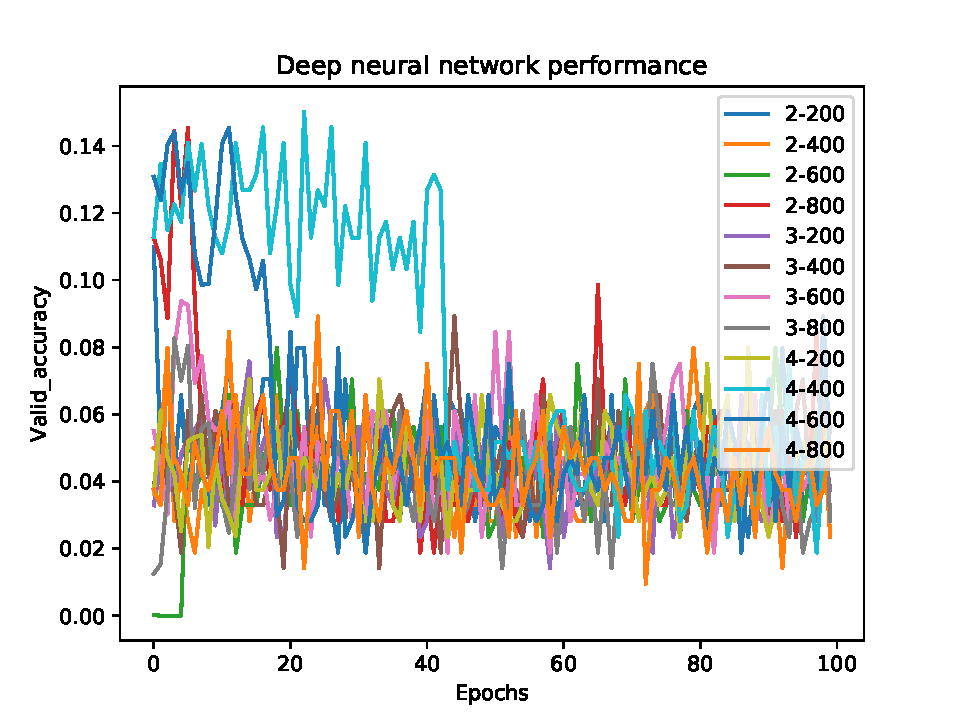
\includegraphics[height=1.25in]{Figs/AL_Valid_accuracy_plots_L2_N3.pdf}}%
\qquad
\caption{The error and accuracy curves of both training and validation sets with full data tested}
\label{fig:fulldata}
\end{figure}

As the Figure.\ref{fig:fulldata} shown, both the error of training set and validation set are increasing, which indicates that there is something wrong and the DNN totally unable to learn the features.

At the beginning, we thought it might be the learning rate problem. However, after we carefully searched, the learning rate have been set to a proper value and the neural network still cannot learn. The results are unacceptable. Even if DNN is not suitable for this task, the error on training set should not increase as the increasing of epochs. Since the DNN worked well in EMINST data set, we believed there should be something wrong with the data set.

After our carefully checking, we noticed the data set is not balanced. As mentioned before, some songs belong to more than one genres. In our data pre-processing procedure, we mapped the multiple genres into new single genre so that we can implement one-hot coding. However, this increase the number of total genres vastly. The original number of genres are 236 in total. After our pre-processing, the total genre number is 4858, which is about 8 times of our input feature dimensions (which is 518 in total.). Therefore, our neural network cannot perform the classifying work. Because the output dimension is even larger than the input dimension. Therefore, we decide to decrease the number of genres.

\subsection{Experiments with reduced data}
To decrease the number of genres without removing any data, we decide to merge the genres. If one song has more than one genres, we only left the first genre it mentioned as its genre. By doing so, we deceased the number of genres from 4858 to 236, which is smaller than the input dimension. With all parameters unchanged, we implement our experiments again on the reduced data set.The results are shown as following:

\begin{figure}[h]%
\centering
\subfigure[Error of Train]{%
\label{fig:lr0.02}%
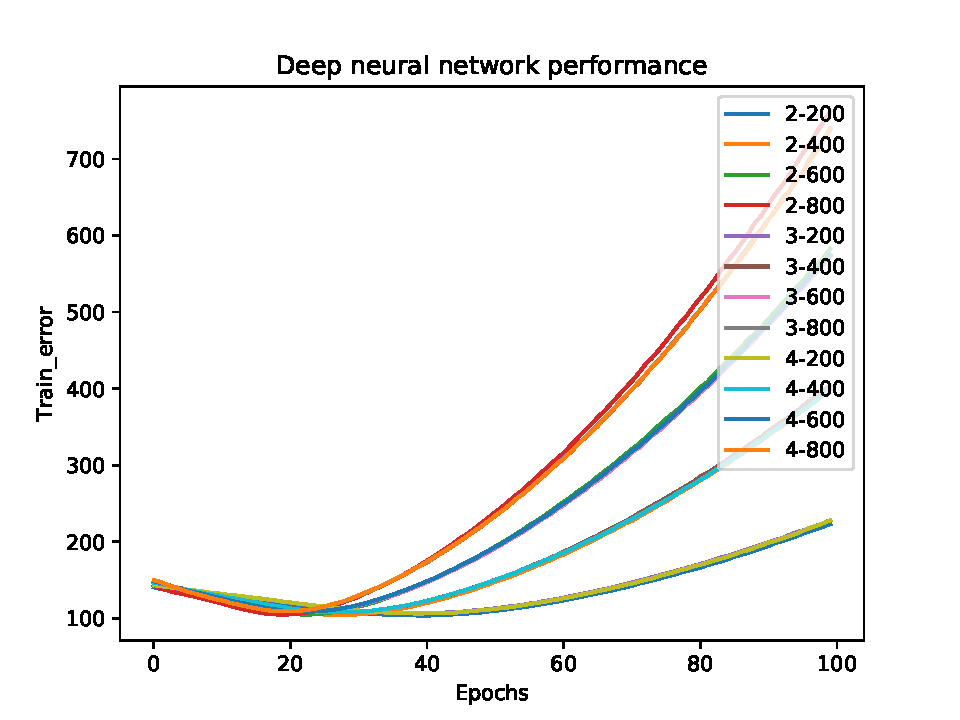
\includegraphics[height=1.25in]{Figs/Re_Train_error_plots_L2_N3.pdf}}%
\subfigure[Accuracy of Train]{%
\label{fig:lr0.04}%
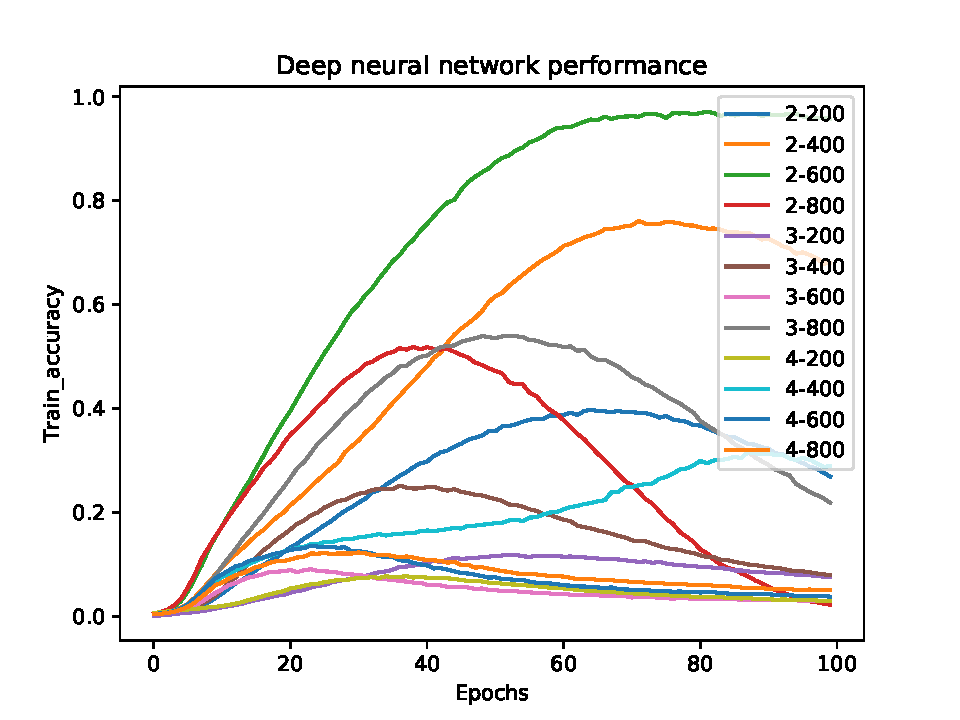
\includegraphics[height=1.25in]{Figs/Re_Train_accuracy_plots_L2_N3.pdf}}%
\qquad
\subfigure[Error of Valid]{%
\label{fig:lr0.06}%
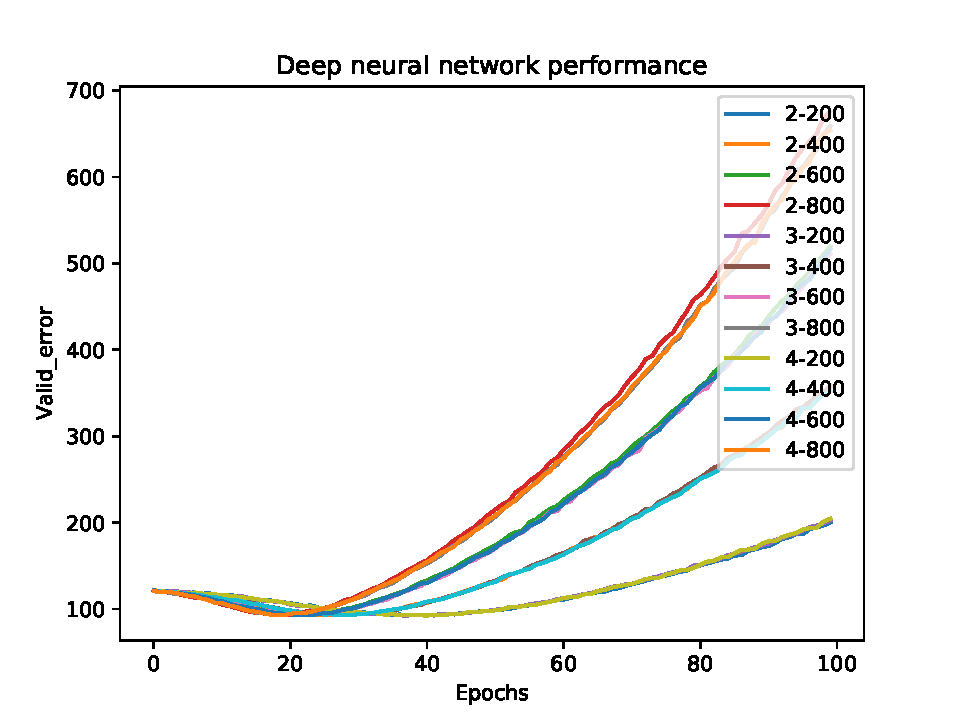
\includegraphics[height=1.25in]{Figs/Re_Valid_error_plots_L2_N3.pdf}}%
\subfigure[Accuracy of Valid]{%
\label{fig:lr0.08}%
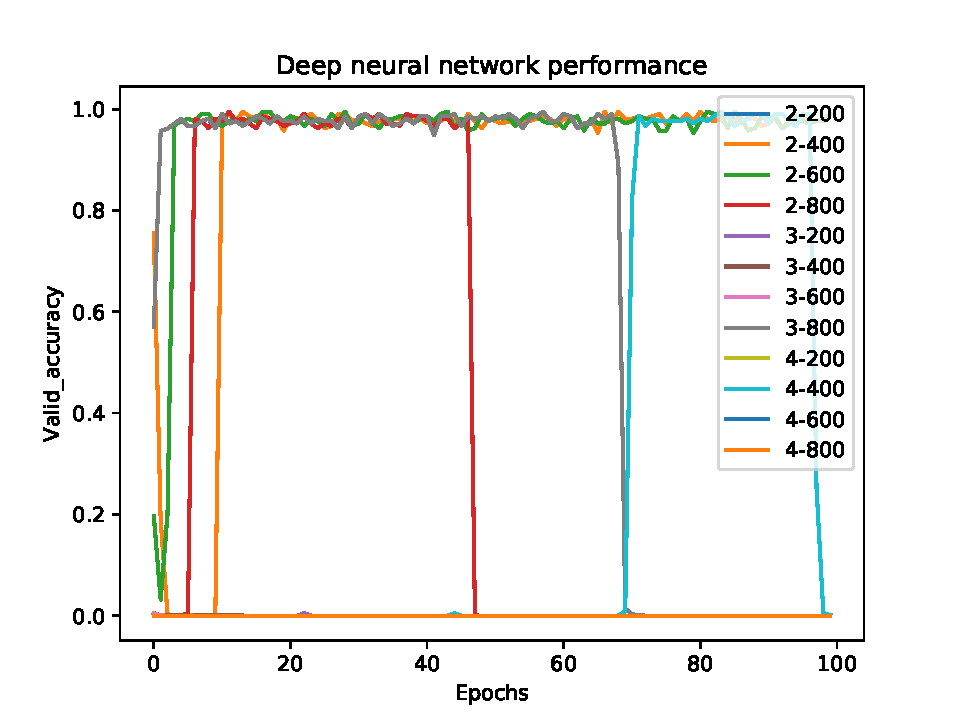
\includegraphics[height=1.25in]{Figs/Re_Valid_accuracy_plots_L2_N3.pdf}}%
\qquad
\caption{The error and accuracy curves of both training and validation sets with reduced data tested}
\label{fig:reduceddata}
\end{figure}

As the Figure.\ref{fig:reduceddata} shown. The results are still quiet bad. By looking at the error of training set, we can infer that there is still something wrong with the data set. Although the error of training set is decreasing at the beginning, it is also increasing at the end. We think no matter how bad the neural network is in dealing with the classifying work, the error of training set should not increase at any time.

Meanwhile, the accuracy of validation set is quite interesting. Some of the situation, the accuracy of validation set is suddenly increased to about 1 (100$\%$ accuracy) and suddenly decreased to zero again. We guessing this is because when we cutting the data, there is something wrong with our shuffle process which cause the data in validation set is not shuffled. Therefore, since only one or two genres in the validation set, the accuracy rate will be look like this.

Later, we found that we forgot to shuffle the reduced validation set. Due to the time limitation, we cannot implement this experiments again. However, since we shuffle the data separately, other data sets are not affected.

After testing with various learning rates and other parameters, we thought it is still the data set problem. Inspired by EMINST data set (which input dimension is 20 times to output dimension) and MINST data set (which input dimension is 70 times to output dimension), we decide to decrease the number of genres even more.

\subsection{Experiments with deleted data}
Since we have reduced the data set, it is impossible to decrease the number of genres without deleting data. Therefore, we decide to use the top 10 genres in the data set. If a song is not belong to one of the top 10 genres, we will delete it from the data set. By constructing our data set in this way, we decreased the number of genres to 10 with saving most of the data.With all parameters unchanged, we implement our experiments again on the deleted data set.The results are shown as following:

\begin{figure}[h]%
\centering
\subfigure[Error of Train]{%
\label{fig:lr0.02}%
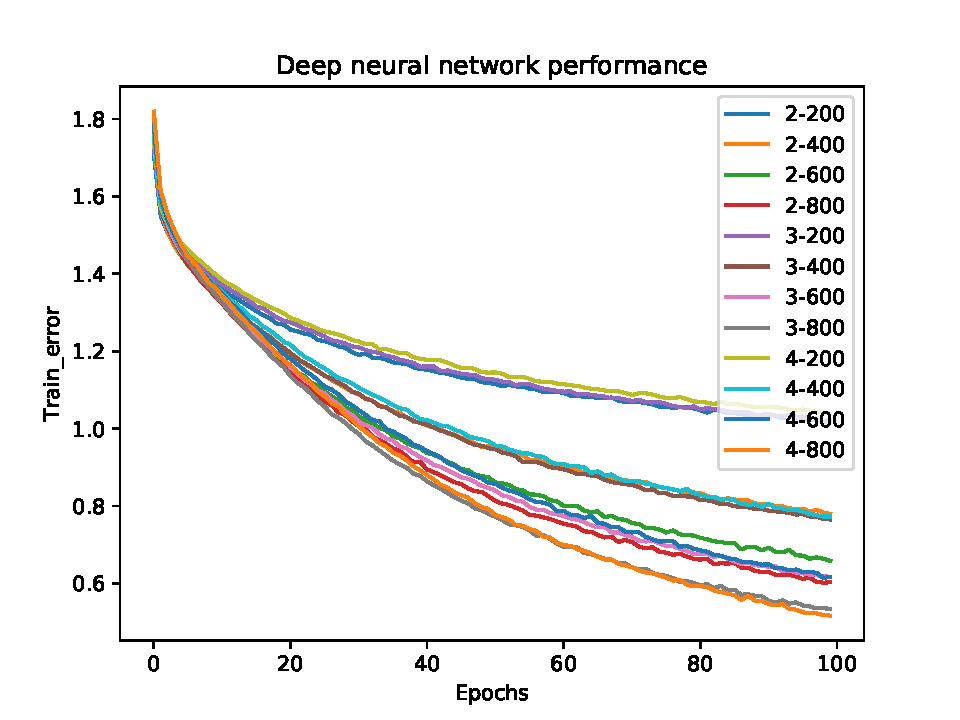
\includegraphics[height=1.25in]{Figs/Ab_Train_error_plots_L2_N3.pdf}}%
\subfigure[Accuracy of Train]{%
\label{fig:lr0.04}%
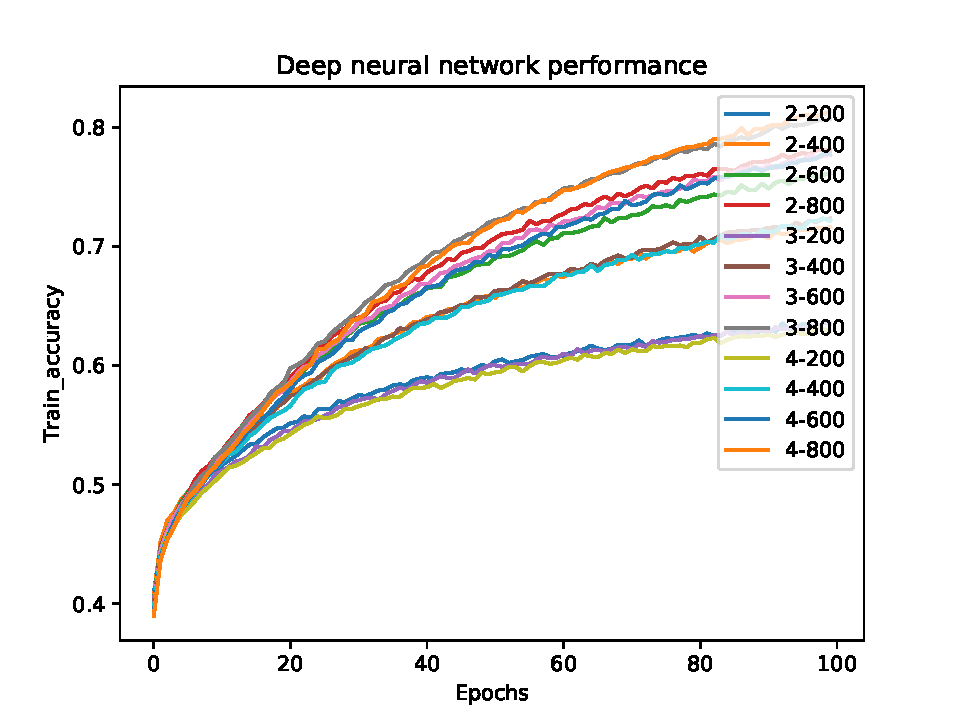
\includegraphics[height=1.25in]{Figs/Ab_Train_accuracy_plots_L2_N3.pdf}}%
\qquad
\subfigure[Error of Valid]{%
\label{fig:lr0.06}%
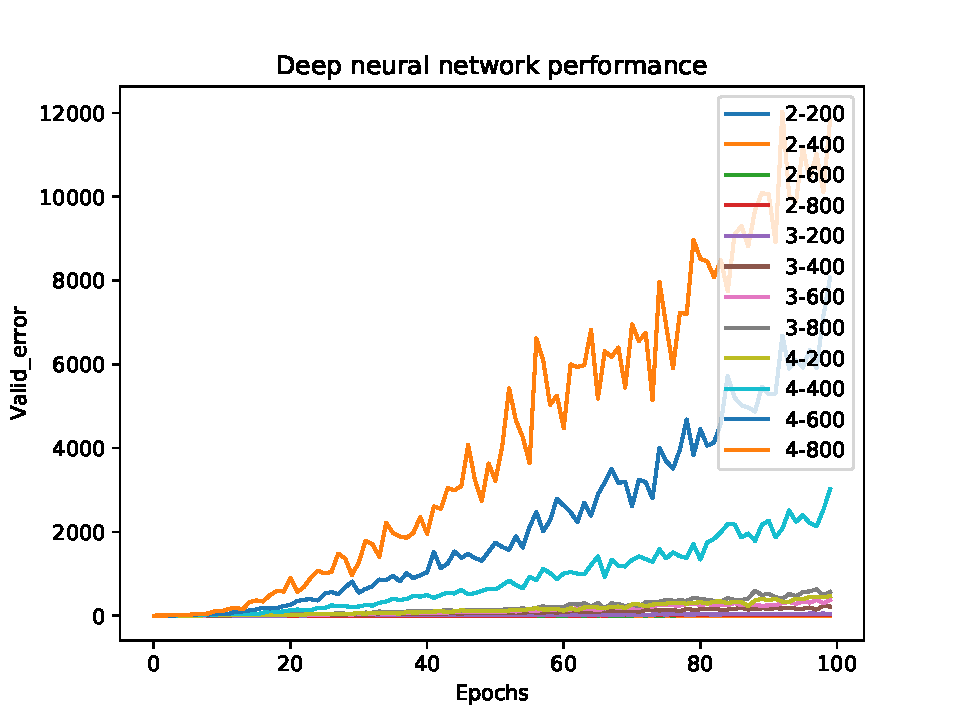
\includegraphics[height=1.25in]{Figs/Ab_Valid_error_plots_L2_N3.pdf}}%
\subfigure[Accuracy of Valid]{%
\label{fig:lr0.08}%
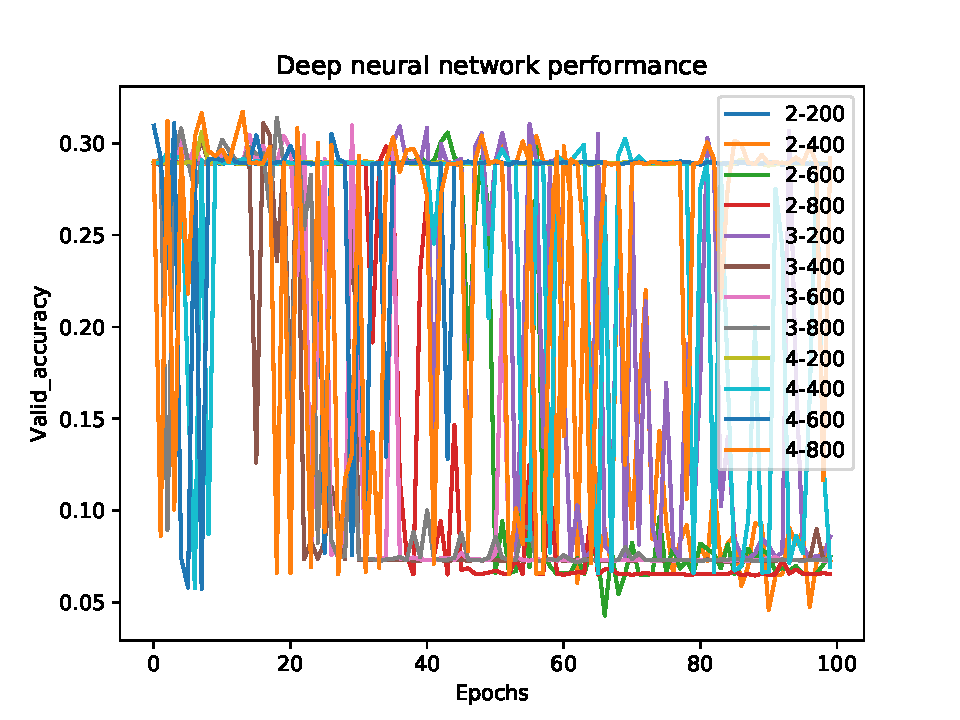
\includegraphics[height=1.25in]{Figs/Ab_Valid_accuracy_plots_L2_N3.pdf}}%
\qquad
\caption{The error and accuracy curves of both training and validation sets with deleted data tested}
\label{fig:deleteddata}
\end{figure}

As the Figure.\ref{fig:deleteddata} shown. The results are finally normal. The error on the training set keeps decreasing and the accuracy on the training set keeps increasing. Which indicates that our neural network model is working with the data set. Which means that our guessing before was right.

However, the results also shows that the data set has another problem. As the error of the validation set keeps increasing rapidly, it is clear that our neural network overfitted to the training data very quickly. What is worse, from the accuracy of the validation set keeps shaking around rather than getting worse, it is clear that the inputs are not quite related to the outputs. In another word, the features in the metadata is not related to the genres of the songs.

In conclusion, during our baseline experiments, we found that the features provided by the FMA project has no strong relationship with the genre of the song. What is worse, the features provided by FMA also have no relationship to time, which means it is hard for us to implement convolutional neural network on this data set. Therefore, we will implement our own music feature function to obtain the features from music files directly and re-implement our experiments with other neural network such as RNN, LSTM and 1-D convolutional neural network.


\section{Interim conclusions}
In this paper, we tried to implement a DNN to build a music classification system, using fma dataset which is a well-constructed data with millions of songs and rich metadata, and proposed to improve the performance of classification accuracy with some data preprocessing. The network contained dropout layer and batch normalization, using sigmoid function and softmax function as activation functions of hidden layers and output layer respectively. The model changed the number of layers and the neurons in each layer to explore the feasibility of the dataset. Due to the extremely many genres to classify, the DNN performed an unreasonable result on the original metadata with increasing error and decreasing accuracy via epochs. Then, we constrained the classes of each song into a single genre but still obtain an unacceptable result. 
In order to achieve a reasonable result, we reduce the classification challenge of the model by only remaining the top-ten-genre songs in the dataset and the model managed to give a more explainable result. The error of validation set increasing rapidly from 0 demonstrated that the model was overfitted in the training stage so when changing another set it performed an unreliable behaviour. From the shaking accuracy of the validation set, we figured out that the limited features of the metadata were not able to classify so many genres or the features had no relation to the genres so the DNN performed such unexplainable results using the features. In the future, we suggest taking the original audio data as the input, which contains the large scale of features and has more relations to the genres.

\section{Plan}
Based on the baseline model we described in the report, we propose to take the following plans to improve the performance of such music classification task and build a reliable system in the future. Due to the incompleteness of the metadata in this music classification task, we are planning to extract data from the original audio files initially, to build a powerful dataset with a vest of parameters in a time sequence. Mel-frequency cepstral coefficients (MFCC) is the commonly used technique to preprocess the audio data for several audio processing tasks \cite{rabiner1993fundamentals}, which not only provides enough parameters of the song but also limits the data to an acceptable scale. 

Then, we will implement different models like long short-term memory (LSTM) \cite{sundermeyer2012lstm}, CNN \cite{lawrence1997face}, recurrent neural network (RNN) \cite{medsker2001recurrent}, etc., to explore a better construction of the neural network to do music classification. To the best of our knowledge, adopting these complicated networks on the fma dataset is rarely reported, so it is still an attractive task. 

It is also a potential choice for us to build a music recommend system if we finally try different networks on the dataset and achieve an acceptable performance. Besides these, optimization for parts of or the whole project will be done depending on relative condition.
 

\bibliography{ref}

\end{document} 


% This document was modified from the file originally made available by
% Pat Langley and Andrea Danyluk for ICML-2K. This version was
% created by Lise Getoor and Tobias Scheffer, it was slightly modified  
% from the 2010 version by Thorsten Joachims & Johannes Fuernkranz, 
% slightly modified from the 2009 version by Kiri Wagstaff and 
% Sam Roweis's 2008 version, which is slightly modified from 
% Prasad Tadepalli's 2007 version which is a lightly 
% changed version of the previous year's version by Andrew Moore, 
% which was in turn edited from those of Kristian Kersting and 
% Codrina Lauth. Alex Smola contributed to the algorithmic style files.  